\section{Adaptive Q-Band Suppression Controller}

\subsection{Band-Energy Projection}
Let the prediction horizon contain $N$ samples and sampling time $\Delta t$. The predicted lateral-acceleration sequence is
\begin{equation}
    \mathbf{A}_y=[a_{y,0},a_{y,1},\ldots,a_{y,N-1}]^\T .
\end{equation}
For a critical band $\mathcal{B}_i$, choose discrete frequencies $f_{ij}$ and time grid $t_k=k\Delta t$. Define
\begin{equation}
    \mathbf{c}_{ij}=[\cos(2\pi f_{ij}t_0),\ldots,\cos(2\pi f_{ij}t_{N-1})]^\T ,
\end{equation}
\begin{equation}
    \mathbf{s}_{ij}=[\sin(2\pi f_{ij}t_0),\ldots,\sin(2\pi f_{ij}t_{N-1})]^\T .
\end{equation}
The band energy is
\begin{equation}
    E_i(\mathbf{A}_y)=\mathbf{A}_y^\T\mathbf{Q}_i\mathbf{A}_y,
\end{equation}
\begin{equation}
    \mathbf{Q}_i=\frac{1}{N^2}\sum_j(\mathbf{c}_{ij}\mathbf{c}_{ij}^\T+\mathbf{s}_{ij}\mathbf{s}_{ij}^\T)\succeq0 .
\end{equation}
The matrix $\mathbf{Q}_i$ can be precomputed for fixed $\Delta t$, $N$, and $\mathcal{B}_i$. Hence the Q-band term adds no new vehicle state; it only reshapes the predicted lateral acceleration.

\subsection{Optimization Problem}
The Q-band ART objective combines tracking, actuator regularization, acceleration smoothing, and band suppression:
\begin{equation}
\begin{aligned}
\min_{\mathbf{U},\mathbf{S}}~&
J_{\mathrm{trk}}+J_u+J_{\Delta u}
w_a\|\mathbf{A}_y\|_2^2+w_1\|\mathbf{D}_1\mathbf{A}_y\|_2^2\\
&+w_2\|\mathbf{D}_2\mathbf{A}_y\|_2^2
\sum_i w_i(t)\mathbf{A}_y^\T\mathbf{Q}_i\mathbf{A}_y
\sum_i\rho_i s_i^2 ,
\end{aligned}
\label{eq:qband_cost}
\end{equation}
where $\mathbf{D}_1$ and $\mathbf{D}_2$ are first- and second-order difference matrices. The constraints are
\begin{equation}
\begin{aligned}
    \mathbf{x}_{k+1}&=f(\mathbf{x}_k,u_k,\hat d_k),\\
    |a_{y,k}|&\leq a_{y,\max}^{\mathrm{dyn}},\\
    u_{\min}&\leq u_k\leq u_{\max},\quad |\Delta u_k|\leq \Delta u_{\max},\\
    E_i(\mathbf{A}_y)&\leq \bar{E}_i+s_i,\quad s_i\geq0 .
\end{aligned}
\label{eq:qband_constraints}
\end{equation}
The soft band constraint prevents the optimizer from concentrating energy in a dangerous band, while preserving feasibility when the reference path is aggressive. In low-risk segments, $w_i(t)$ remains small and the controller behaves like a normal tracker.

\subsection{Preview-Adaptive Scheduling}
Pure feedback scheduling raises the safety weight only after the roll-slosh response has already been excited. Q-band ART uses preview risk as the main trigger. A reference lateral-acceleration sequence $\mathbf{A}_{y,\mathrm{ref}}$ is computed from the future path or curvature, and its band energy is compared with the calibrated threshold:
\begin{equation}
    R_i^{\mathrm{pre}}=\max\left(0,\frac{\mathbf{A}_{y,\mathrm{ref}}^\T\mathbf{Q}_i\mathbf{A}_{y,\mathrm{ref}}}{\bar{E}_{i,\mathrm{ref}}}-1\right).
\end{equation}
The raw weight is scheduled as
\begin{equation}
    w_i^{\mathrm{raw}}=w_i^{\min}+
    \left(1-e^{-\kappa R_i^{\mathrm{pre}}}\right)(w_i^{\mathrm{tar}}-w_i^{\min}).
\end{equation}
Observed yaw or roll residuals can further increase the weight when residual sloshing remains. A non-symmetric filter is then applied:
\begin{equation}
    w_i(t)=(1-\alpha_i)w_i(t-\Delta t)+\alpha_i w_i^{\mathrm{raw}},
\end{equation}
where $\alpha_i=\alpha_\uparrow$ if $w_i^{\mathrm{raw}}>w_i(t-\Delta t)$ and $\alpha_i=\alpha_\downarrow$ otherwise. With $\alpha_\uparrow>\alpha_\downarrow$, the weight rises before a high-risk lane change and decays slowly after it.

\begin{figure}[!t]
\centering
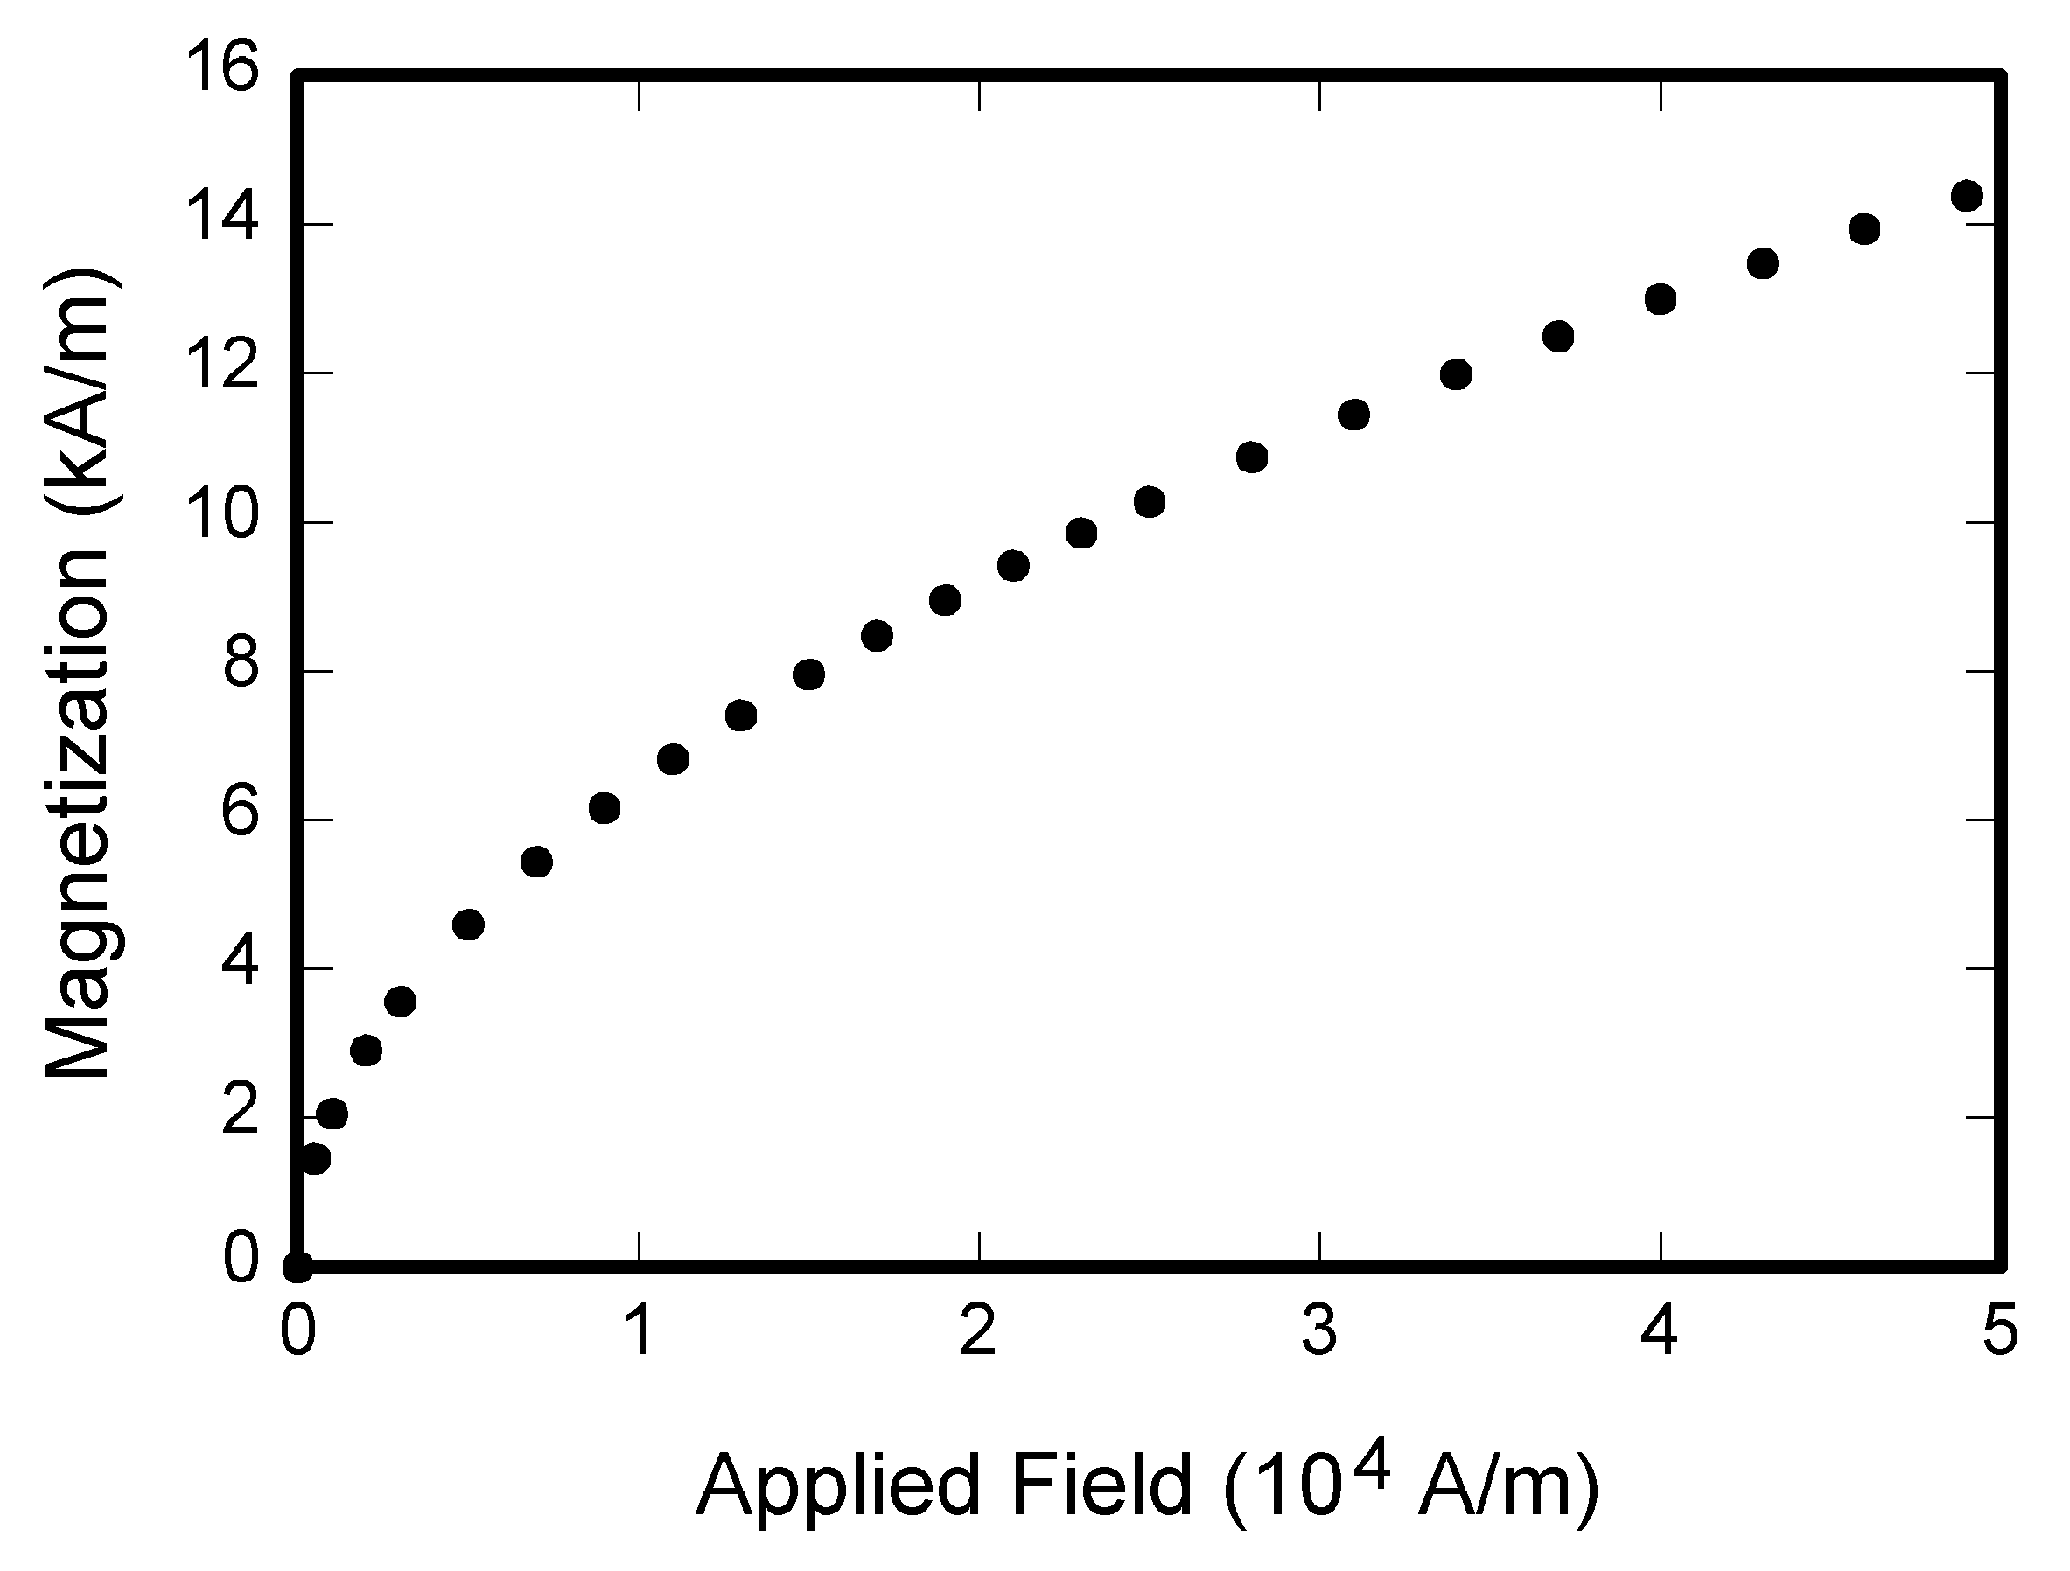
\includegraphics[width=\linewidth]{fig/fig1.png}
\caption{Adaptive Q-band scheduling. Preview risk increases band weights before aggressive steering, while residual monitoring delays weight release after the maneuver.}
\label{fig:qband_scheduler}
\end{figure}
% TODO（作者）：将 fig1.png 替换为自适应权重流程图。建议用少量模块画出 reference preview、band energy、feedback residual、asymmetric smoothing、scheduled weights 和 NMPC。

\subsection{Implementation Notes}
The Q-band module is model-agnostic. For a kinematic predictor, $a_{y,k}$ can be approximated from curvature or steering; for a dynamic predictor, it can be computed from $\dot v_y+v_xr$; for TruckSim or model-truck validation, it is evaluated from the predicted tracking response. In all cases, the controller suppresses the lateral excitation sequence rather than explicitly controlling the liquid state.

% TODO（作者）：后续补充最终控制频率、预测步长、求解器、平均/峰值求解时间、低速 PP 与高速 NMPC 的切换阈值。若篇幅紧张，可放入一行 implementation paragraph。
